\documentclass[dutch]{beamer}
\mode<presentation>

%\documentclass[handout]{beamer}
%\usepackage{pgfpages}
%\pgfpagesuselayout{4 on 1}[a4paper,border shrink=5mm,landscape]
%\setbeamertemplate{footline}[frame number]

\usepackage[dutch]{babel}
\usepackage{graphicx}
\usepackage{amssymb, subfigure}
\usepackage{amsthm}
\usepackage[utf8]{inputenc}
\usepackage[normalem]{ulem}
\usepackage{color}
\usepackage{cancel}

\newcommand{\vraag}[1]{\begin{itemize}\item {\it #1}\end{itemize}}
\newcommand{\degree}{\ensuremath{^\circ}}

\graphicspath{{../figuren/}}

\begin{document}
\small

\begin{frame}
 \frametitle{Iets statistisch onderzoeken}
 {\it Onderzoeken} is iets nauwkeurig nazien of nagaan.\\
 {\bf Onderzoeksvraag}: vraag die bij een onderzoek hoort.\\
 {\it Statistisch onderzoek} is een onderzoek die verloopt volgens de statistiek.\\
 {\bf Statistiek} is de wetenschap van het waarnemen van verschijnselen en het weergeven van de uitkomsten in getallen en figuren.\\
 Onderzoek:\\
 \begin{enumerate}
  \item Wat wil je weten? Hoe ga je meten?
  \item Op speurtocht gaan in de dataset.
  \item Wat heb je gevonden? Hoe ver kan je gaan in je conclusie?
  \item Kernachtig samenvatten van onderzoek.
\end{enumerate}
\end{frame}

\begin{frame}
\frametitle{Statistisch onderzoek naar de kleuren van M\&M-snoepjes}
{\bf Onderzoeksvraag:}\\
Heb je enig idee welke kleuren allemaal voorkomen bij M\&M’s?
Komt elke kleur evenveel voor?\\\vspace*{0.5cm}

{\bf Populatie} als je “de totale verzameling” bedoelt.\\
{\bf Steekproef} is een deeltje van een populatie.\\\vspace*{0.5cm}

{\bf Aselecte steekproef}: goed mengen en dan lukraak snoepjes eruit nemen.\\
{\bf Aselect} zijn: elk element van de populatie moet dezelfde kans hebben om opgenomen te worden tot de steekproef.\\
{\bf Representatief} zijn: de steekproef een correct beeld moet geven van de verscheidenheid binnen de populatie.\\
{\bf steekproefgrootte}: aantal gekozen snoepjes.

\end{frame}

\begin{frame}
\frametitle{Gegevensverzameling of dataset}
De {\bf elementen} zijn de objecten die in een statistische studie worden onderzocht (de snoepjes).\\
Elke {\bf veranderlijke} is één welbepaalde eigenschap die je opmeet (de kleur).\\
{\bf Kwalitatieve veranderlijke}: veranderlijke waarop geen zinvolle wiskundige bewerkingen uitgevoerd kunnen worden.\\ 
De {\bf dataset} is een tabel met op de rijen de elementen en in de kolommen de veranderlijken.\\
\vraag{Maak een tabel waarin je de gegevens zal opschrijven. Als je afkortingen gebruikt, schrijf dan ook op wat die afkortingen betekenen.}
\vspace{5cm}
\end{frame}

\begin{frame}
\frametitle{Frequentietabel}
\vraag{Gebruik je dataset om een frequentietabel op te stellen.}
\begin{center}
  \begin{tabular}{|p{2cm}|p{2cm}|p{2cm}|}
    \hline
    \uncover<2->{Kleur}&\uncover<2->{Frequentie}&\uncover<5->{Relatieve Frequentie}\\
    \hline
    &&\vspace*{0pt}\\
    \hline
    &&\vspace*{0pt}\\
    \hline
    &&\vspace*{0pt}\\
    \hline
    &&\vspace*{0pt}\\
    \hline
    &&\vspace*{0pt}\\
    \hline
    &&\vspace*{0pt}\\
    \hline
  \end{tabular}
\end{center}
%\vspace{1cm}
\uncover<3->{\vraag{Hoe kan je de steekproefgrootte snel berekenen met behulp van de frequentietabel?}}
\uncover<4->{\underline{Tel alle frequenties samen} want dan heb je het totale aantal snoepjes en dat is gelijk aan de
steekproefgrootte.}
\end{frame}

\begin{frame}
\frametitle{Relatieve frequentie}
\vraag{Als er in de volledige populatie, dus alle snoepjes in het vat, 6 kleuren zitten. En
van elk kleur zijn er evenveel snoepjes. Wat is dan de kans om lukraak een geel snoepje te kiezen?}
\pause
Van elk kleur zijn er evenveel snoepjes. Dus \uline{elk kleur heeft evenveel kans om gekozen te worden}. Er zijn zes kleuren, dus de kans is $\frac{1}{6}$.
\pause
\vraag{De relatieve frequentie voor "geel" wijkt af van de theoretische kans, verklaar dit en wanneer
zou de relatieve frequentie dichter bij de theoretische kans moeten komen?}
\pause
De relatieve frequentie werd berekend uit een steekproef. \uline{Een steekproef is een lukraak deel van de volledige populatie}. \uline{Hoe groter de steekproef}, hoe dichter we bij de volledige populatie komen en hoe dichter we bij de theoretische kans komen.
\end{frame}

\begin{frame}
\frametitle{Staafdiagram}
Het {\bf Staafdiagram} is de basisfiguur voor kwalitatieve veranderlijken.
Werkwijze:
\begin{enumerate}
  \item Op de $x$-as zet je de verschillende kleuren.
\item Op de $y$-as duid je de frequentie van elke kleur aan en je tekent dan bij elke kleur een staafje
waarvan de lengte overeenkomt met de frequentie van die kleur. Zorg ervoor dat alle staafjes
los van elkaar staan.
\item Voorzie de assen van de juiste naam.
\end{enumerate}
\pause
\vraag{Teken nu zo’n staafdiagram voor het onderzoek.}
\end{frame}


\begin{frame}
\frametitle{Taartdiagram}
Het {\bf Taartdiagram} is bij uitstek bruikbaar om de relatieve frequentie weer te geven.\\
Eén stukje uit een taartdiagram heet een {\bf sector}.\\
Afspraken:
\begin{itemize}
  \item Begin bovenaan en draai met de wijzers van de klok mee.
  \item De grootste sector komt eerst, dan komt de tweede
grootste, enzovoort.
\end{itemize}
\pause
\vraag{Bereken eerst voor elke relatieve frequentie hoe groot de sector is die daarbij hoort.}
\begin{center}
  \begin{tabular}{|p{1cm}|p{1cm}|p{1cm}|p{1cm}|p{1cm}|p{1cm}|p{1cm}|}
    \hline
    kleur:\vspace{0.5cm}&&&&&&\\
    \hline
    hoek:\vspace{0.5cm}&&&&&&\\
    \hline
  \end{tabular}
\end{center}
\pause
\vraag{Teken nu cirkelsectoren die overeenstemmen met de relatieve frequenties.}
\end{frame}

\begin{frame}
\frametitle{Variabiliteit van de steekproefresultaten}
Laten we nu eens kijken naar de inhoud van een aantal andere zakjes M\&M's.\\
\pause
\vraag{Verwacht je dat de andere zakjes dezelfde resultaten zullen hebben als het eerste zakje?}
\pause
\uline{Neen}. Er is \uline{fluctuatie} bij het vullen van de zakjes en dus zullen de antwoorden niet identiek
zijn. Waarschijnlijk lijken de antwoorden wel goed op elkaar, maar anderzijds krijg je snel
“schijnbaar” grote verschillen bij zo’n kleine aantallen. Als er toevallig in een zakje 4
bruine snoepjes zitten en in een ander zitten er 8 bruine, dan is dat plots dubbel zoveel.
\pause
\vraag{Kan je je antwoord op vorige vraag wat verduidelijken door te verwijzen naar de manier
waarop die zakjes gevuld worden? Kan je hierbij ook de woorden populatie en steekproef op
een juiste wijze gebruiken?}
\pause
\uline{Elk zakje kan je beschouwen als een nieuwe steekproef} uit dezelfde grote populatie van alle
M\&M’s. Bij \uline{een steekproef trek je lukraak} en het is dus normaal dat de resultaten van de ene
steekproef niet identiek dezelfde zijn als de resultaten van een andere steekproef.
\end{frame}

\begin{frame}
\frametitle{Variabiliteit van de steekproefresultaten}
In plaats van naar alle kleuren te kijken, zou je er eens je lievelingskleur kunnen uithalen,
bijvoorbeeld blauw.\\
\pause
\vraag{Noteer voor elk onderzocht zakje telkens het percent blauwe snoepjes.}
\vspace*{1cm}
\pause
\vraag{Als jij maar één zakje snoepjes mag onderzoeken (bijvoorbeeld het eerste) en je zou moeten raden hoeveel
percent blauwe snoepjes er door de fabrikant gemaakt wordt (dus hoeveel percent blauwe
snoepjes er in de totale populatie zit), wat zou jij dan antwoorden?}
\vspace*{1cm}
\pause
\vraag{Is je bovenstaand antwoord exact juist? Hoe weet je dat?}
\pause
Neen, want een ander zakje kan een ander aantal blauwe snoepjes bevatten. \uline{Een steekproefuitslag is nooit "wiskundig exact"}! We kunnen enkel een benadering geven.
\end{frame}

\begin{frame}
\frametitle{Steekproefgrootte, nauwkeurigheid en haalbaarheid}
Het is beter om met een grotere steekproef te werken dan met een kleinere. Om een grotere steekproef te krijgen brengen we nu alle open gedane zakjes M\&M's samen en gebruiken we deze als één grote steekproef.
\vraag{De verschillende resultaten van elk onderzocht zakje worden nu verzameld.}
\begin{center}
  \begin{tabular}{|p{2cm}|p{2cm}|p{2cm}|}
    \hline
    Kleur&Frequentie&Relatieve frequentie\\
    \hline
    &&\vspace*{0pt}\\
    \hline
    &&\vspace*{0pt}\\
    \hline
    &&\vspace*{0pt}\\
    \hline
    &&\vspace*{0pt}\\
    \hline
    &&\vspace*{0pt}\\
    \hline
    &&\vspace*{0pt}\\
    \hline
  \end{tabular}
\end{center}
\end{frame}

\begin{frame}
\frametitle{Een model voor de populatie}
Bij M\&M’s komen alle kleuren globaal (in de populatie) evenveel voor.

\vraag{Maak een tabel waarin je aangeeft hoe de populatie er precies uitziet. Gebruik je frequenties
of relatieve frequenties in die tabel?}
\begin{center}
  \begin{tabular}{|p{2cm}|p{2cm}|}
    \hline
    Kleur&\\
    \hline
    &\vspace*{0pt}\\
    \hline
    &\vspace*{0pt}\\
    \hline
    &\vspace*{0pt}\\
    \hline
    &\vspace*{0pt}\\
    \hline
    &\vspace*{0pt}\\
    \hline
    &\vspace*{0pt}\\
    \hline
  \end{tabular}
\end{center}
\end{frame}

\begin{frame}
\frametitle{Een staafdiagram met subgroepen}
\vraag{Hoe ga je de grafiek tekenen? Welke volgorde kies je voor de kleuren op de $x$-as?}
\pause
Om twee situaties met elkaar te vergelijken, ga ik met \uline{relatieve frequenties} werken. Enkel als
ik toevallig even grote subgroepen zou hebben, zou ik ook frequenties kunnen gebruiken.
Voor het staafdiagram met subgroepen plaats ik de \uline{kleuren op de x-as} en de \uline{relatieve
frequenties op de y-as}. Omdat de kleuren van de populatie hier allemaal dezelfde relatieve
frequentie hebben mag ik de volgorde vrij kiezen. Ik zou mij daarbij kunnen laten leiden door
de relatieve frequenties in de steekproef.
\pause
\vraag{Teken nu de grafiek.}
\pause
\vraag{Kan je verklaren waarom jouw cijfers eventueel afwijken van die van de fabrikant?}
\pause
De \uline{cijfers van de fabrikant liggen vast}, want zij beschrijven het model van de totale
populatie. De \uline{cijfers van mijn klas zijn toevallige uitkomsten van een steekproef}. Als wij
volgende week een nieuw onderzoek van M\&M’s zouden doen, dan zouden wij waarschijnlijk
andere resultaten vinden voor onze klas. Maar de cijfers van de fabrikant veranderen niet.
\end{frame}

\begin{frame}
\frametitle{Kernachtige samenvatting van dit onderzoek}
\begin{itemize}
  \item Informatie over het onderzoek.
  \item Antwoorden op de contextvragen.
  \item Besluiten over het uitgevoerde onderzoek.
\end{itemize}
\pause
De contextvragen:
\begin{enumerate}
  \item {\bf Waarom} is dit onderzoek uitgevoerd?
  \item {\bf Waar} is dit onderzoek uitgevoerd?
  \item {\bf Wanneer} is dit onderzoek uitgevoerd?
  \item {\bf Wie of wat} wordt onderzocht?
  \item {\bf Wat} wordt er juist opgemeten?
  \item {\bf Hoe} wordt dit onderzoek uitgevoerd?
\end{enumerate}
\end{frame}

\begin{frame}
\frametitle{Antwoorden op contextvragen}
\vraag{Formuleer in een bondige tekst de antwoorden op de contextvragen.}
\pause
Op \uline{maandag 23 april 2012} hebben we in \uline{onze school} tijdens de les wiskunde een
onderzoek gedaan naar de \uline{kleuren van M\&M-snoepjes}. We wilden weten \uline{welke kleuren}
allemaal voorkwamen en \uline{hoe vaak elke kleur} voorkomt. Voor dit onderzoek hebben we een
aantal zakjes M\&M gebruik. We hebben ook \uline{met de gegevens van de fabrikant rekening gehouden}.
We wilden namelijk de resultaten van onze toevallige steekproef vergelijken met de
populatie-eigenschappen die de fabrikant opgeeft.
\end{frame}

\begin{frame}
\frametitle{Besluiten over het onderzoek}
\vraag{Formuleer in een bondige tekst je besluiten over het uitgevoerde onderzoek.}
\pause
Bij het onderzoeken van de kleuren van M\&M’s hebben we vastgesteld dat er \uline{in elk zakje
dezelfde kleuren voorkomen}, maar \uline{niet allemaal in dezelfde hoeveelheid}. Dit is te verklaren
omdat \uline{zakjes lukraak gevuld} worden. Elk zakje kan beschouwd worden als een lukrake
steekproef uit een enorm grote populatie. Als we alle \uline{zakjes samenvoegen, dan hebben we
een grotere steekproef} maar ook die is te beschouwen als een lukrake steekproef van snoepjes
uit de grote populatie. Het is dus te verwachten dat onze resultaten niet exact samenvallen
met de cijfers die de fabrikant opgeeft.
\end{frame}

\begin{frame}
\frametitle{Zelfevaluatie}
In dit onderzoek heb je geleerd over:\\
\begin{itemize}
  \item de context van een statistisch onderzoek (wanneer, waar,...)
  \item het onderscheid tussen de populatie en een steekproef
  \item een aselecte steekproef
  \item de structuur van een dataset (elementen, veranderlijken)
  \item kwalitatieve veranderlijken
  \item de frequentietabel bij een kwalitatieve veranderlijke
  \item het staafdiagram bij een kwalitatieve veranderlijke
  \item het taartdiagram bij een kwalitatieve veranderlijke
\end{itemize}
\end{frame}

\begin{frame}
\frametitle{Opdrachten}
\vraag{Zeg in eigen woorden op welke vragen je een antwoord moet kunnen geven als men vraagt
naar de context van een statistisch onderzoek.}
\pause
Een verslag moet samen met de bedoeling (waarom?) van een statistisch onderzoek ook de
omstandigheden vermelden waarin dit onderzoek is uitgevoerd. Dat betekent dat je plaats
(waar?) en tijd (wanneer?) moet aangegeven, samen met de manier waarop de steekproef is
getrokken (hoe?) en wat er daarna bij wie is opgemeten.
\pause
\vraag{Omschrijf de begrippen steekproef en populatie in je eigen woorden en geef een (nieuw)
voorbeeld. Leg voor jouw voorbeeld uit hoe je daar een aselecte steekproef zou
trekken.}
\pause
Een populatie is het grote geheel waarover je iets wil weten. Een steekproef is een klein
deeltje uit die populatie. Als ik wil weten of 14-jarige Vlaamse jongeren voor of tegen
huiswerk zijn, dan bestaat de populatie die ik onderzoek uit alle 14-jarige Vlaamse jongeren.
Om hieruit een enkelvoudige aselecte steekproef te trekken, zou ik al die jongeren een
nummer geven en dan 100 toevalsgetallen gebruiken om een steekproef van 100 jongeren te
trekken. In de praktijk is dit geen eenvoudige opdracht.
\end{frame}

\begin{frame}
\frametitle{Opdrachten {\smallskip (vervolg)}}
\vraag{Leg duidelijk uit hoe een dataset eruitziet. Gebruik hiervoor een nieuw voorbeeld dat je zelf
hebt bedacht.}
\pause
In een dataset verzamel je de onderzoeksgegevens. Per onderzochte persoon (of voorwerp)
maak je een rij in een tabel. Dit zijn de elementen. Bij elk element meet je één of meerdere
dingen op. Dit zijn de veranderlijken. Die worden in de kolommen geschreven.
Als je wil weten wat het merk is van de lievelingsfrisdrank van de leerlingen van je school,
dan kan je eerst een lukrake steekproef van 30 leerlingen trekken. Dat zijn de elementen van
je dataset en dus de 30 rijen in je tabel. Per leerling kan je dan bijvoorbeeld de naam, de klas
en het merk noteren. Dat zijn dan 3 veranderlijken per element en die komen in de 3
kolommen van je dataset terecht.
\pause
\vraag{Zeg in eigen woorden wanneer je over een kwalitatieve veranderlijke spreekt. Is de bloedgroep zo’n veranderlijke? Kan je zelf een kwalitatieve veranderlijke bedenken?}
\pause
Een kwalitatieve veranderlijke is een veranderlijke waarmee met de mogelijke uitkomsten
geen zinvolle wiskundige bewerkingen kunnen gedaan worden. De bloedgroep van een
persoon is een goed voorbeeld van een kwalitatieve veranderlijke.
\end{frame}

\begin{frame}
\frametitle{Horizontaal staafdiagram}
\begin{center}
  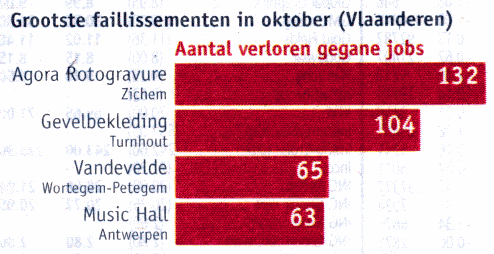
\includegraphics[width=0.6\textwidth]{horizontaal_staafdiagram-faillissementen}
\end{center}
\vraag{Welke veranderlijke is er genoteerd bij elke persoon die zijn job is
kwijtgeraakt? Welk soort veranderlijke is dat? Wat zijn haar waarden? Is de figuur goed
getekend?}
\pause
Voor elke persoon die zijn job is verloren, is genoteerd op welk bedrijf hij werkte. De
veranderlijke is hier “de bedrijfsidentificatie”. Dat is een kwalitatieve
veranderlijke met waarden: “Agora Rotogravure, Zichem”, “Gevelbekleding, Turnhout”,
“Vandevelde, Wortegem-Petegem”, en “Music Hall, Antwerpen”. De figuur is een
staafdiagram waarbij de volgorde van de staafjes bepaald is door de frequentie. Dat is goed.
\end{frame}


\end{document}




























